\documentclass[a4paper,12pt]{article}

\usepackage[utf8]{inputenc}
\usepackage[T1]{fontenc}
\usepackage[ngerman]{babel}
\usepackage{graphicx}
\usepackage{amsmath,amsthm, amssymb}
\usepackage{mathtools}
\usepackage{xcolor}
\usepackage{minted}
\usepackage{lmodern}
\usepackage[a4paper,margin=2.5cm]{geometry}
\usepackage{fancyhdr}
\usepackage{setspace}
\usepackage{caption}
\usepackage{subcaption}
\usepackage{nicefrac}
\usepackage{hyperref}

\usemintedstyle{colorful}
\definecolor{bg}{rgb}{1,1,1}

\pagestyle{fancy}
\fancyhf{}
\lhead{PS Einführung in die Kryptographie}
\rhead{Andreas Schlager}
\cfoot{\thepage}

\title{Aufgabenblatt 06\\\large PS Einführung in die Kryptographie}
\author{Andreas Schlager}
\date{\today}

\onehalfspacing

% Theorem-Umgebung für Aufgaben
\newtheorem{aufgabe}{Aufgabe}

% ---- Makro für neue Aufgabe ----
\newcommand{\newaufgabe}[1]{
  \newpage
  \begin{aufgabe}
  #1
  \end{aufgabe}
  \addcontentsline{toc}{section}{Aufgabe \theaufgabe}
}

\begin{document}

\maketitle
\tableofcontents
\newpage

% Startnummer anpassen (z.B. erste Aufgabe hat Nummer 20, dann counter auf 19 setzen)
\setcounter{aufgabe}{20}

% ---- Aufgaben ----
\newaufgabe{Fortsetzung Aufgabe 20.): Erklären sie, warum die Verwendung von Hashfunktionen
im Kontext mit digitalen Signaturen die Protokollattacke gegen digitale Empfangsbestätigungen verunmöglicht. Bedenken sie dabei insbesondere, dass in diesem Fall
NachrichtenHash und Nachricht übermittelt werden (die Fragen in Item 2 auf Skriptum S. 93 müssen bearbeitet werden).}
Sei $m$ die Nachricht, die Alice an Bob übermitteln möchte. Alice verschlüsselt 
die Nachricht mit Bobs öffentlichem Schlüssel und sendet ihm $E_B(m)$. 
Zusätzlich erzeugt sie den Hashwert $h(m)$ mittels einer kryptografischen 
One-Way-Hashfunktion, signiert diesen mit ihrem privaten Schlüssel und 
verschlüsselt auch die Signatur mit Bobs öffentlichem Schlüssel:
\[
    \begin{rcases}
        E_B(m)\\
        E_B(S_A(h(m)))
    \end{rcases}
    \rightarrow \text{Bob}
\]
Bob entschlüsselt beide Nachrichtenkomponenten, extrahiert den Klartext $m$ 
sowie die Signatur $S_A(h(m))$, und berechnet anschließend selbst den Hashwert 
$h(m)$. Anschließend überprüft er die Signatur mit Alices öffentlichem Schlüssel. 
Stimmen der berechnete Hash $h(m)$ und der signierte Hash überein, ist die 
Integrität der Nachricht sichergestellt.

Im Anschluss sendet Bob eine digitale Empfangsbestätigung zurück. Diese besteht 
nicht aus einer Signatur der vollständigen Nachricht, sondern aus der Signatur 
des Hashwerts:
\[
    E_A(S_B(h(m)))
\]
Eine Protokollattacke, wie sie in Aufgabe 20 beschrieben wurde, ist in diesem 
Szenario nicht mehr möglich. Grund hierfür sind die 
Eigenschaften der verwendeten Hashfunktion:
\begin{itemize}
    \item \textbf{Kollisionsresistenz:} Es ist praktisch nicht möglich, zwei verschiedene Nachrichten $m \neq m'$ zu finden, sodass $h(m) = h(m')$ gilt.
    \item \textbf{Pre-Image-Resistenz:} Aus einem gegebenen Hashwert $h(m)$ kann keine gültige Nachricht $m$ rekonstruiert werden.
\end{itemize}
Selbst wenn Mallory die Nachrichtenkomponenten vom 
ursprünglichen Protokollangriff kennt und in der Lage wäre, die Signaturen und 
Verschlüsselungen zu trennen, fehlt ihm dennoch die Möglichkeit, aus dem Hashwert 
$h(m)$ die Originalnachricht $m$ zu rekonstruieren oder eine alternative Nachricht 
$m'$ mit demselben Hash zu erzeugen.
Somit verhindert die Einbindung von One-Way-Hashfunktionen diese Art der 
Attacken gegen digitale Empfangsbestätigungen.
\newaufgabe{HÜ10 auf S. 86 der VO-Slides.}
\paragraph{Fall 1} Sei $M$ eine beliebige, aber fixe Nachricht zu der eine
Nachricht $M'$ gefunden werden soll, sodass $h(M) = h(M')$. 
Da die Hashfunktion einen $m$-Bit langen Output produziert, gibt es $2^m$ mögliche 
Hashwerte. Die Wahrscheinlichkeit eine entsprechenden Nachricht $M'$ zu generieren ist
\[
P(h(M) = h(M')) = \frac{1}{2^m}.
\]
Das zufällige erzeugen einer Nachricht von Nachricht $M_1,M_2,\dots$
bis der Hashwert übereinstimmt, entspricht einer geometrischen Verteilung.
\[
    \mathbb{E}[N]=\frac{1}{p}=\frac{1}{\frac{1}{2^m}}=2^m
\]
\paragraph{Fall 2} Man berechnet $M_1,M_2,\dots,M_n$ und will wissen wie viele Nachrichten 
man generieren muss, damit es zumindest eine Übereinstimmung der Hashwerte gibt.
Dafür betrachtet man die Gegenwahrscheinlichkeit, dass alle Hashwerte unterschiedlich sind.
\begin{align*}
    \text{\# günstige Fälle} &= 2^m \cdot (2^m - 1) \cdots (2^m - (n - 1))\\
    \text{\# mögliche Fälle} &= (2^m)^n\\
    P(\text{alle unterschiedlich}) &= \frac{2^m}{2^m}\cdot \frac{2^m - 1}{2^m} \cdots \frac{2^m - (n-1)}{2^m}
    =\prod_{k = 0}^{n-1} \left( 1 - \frac{k}{2^m}\right)
\end{align*}
Wir schreiben das Produkt durch den Logarithmus in eine Summe um.
\begin{align*}
    P(\text{alle unterschiedlich}) &= \prod_{k = 0}^{n-1} \left( 1 - \frac{k}{2^m}\right)\\
    \ln P(\dots) &= \sum_{k=0}^{n-1}\ln\left(1-\frac{k}{2^m}\right)
\end{align*}
Da $k \ll 2^m$ kann für $\ln(1-x)$ die Annäherung $\ln(1-x) \approx -x$ getroffen werden.
\[
    \sum_{k=0}^{n-1}\ln\left(1-\frac{k}{2^m}\right) = -\sum_{k=0}^{n-1}\frac{k}{2^m}
    =-\frac{1}{2^m}\sum_{k=0}^{n-1}k=-\frac{1}{2^m}\cdot\frac{n(n-1)}{2}
\]
Für die Gegenwahrscheinlichkeit bedeutet das
\begin{align*}
    \ln P(\text{alle unterschiedlich}) &\approx -\frac{1}{2^m}\cdot\frac{n(n-1)}{2}\\
    P(\text{alle unterschiedlich}) &\approx \exp \left(-\frac{1}{2^m}\cdot\frac{n(n-1)}{2}\right)
\end{align*}
Wir suchen wieder ein $n$ für das $P(\text{alle unterschiedlich}) \approx \nicefrac{1}{2}$, d.h.
\begin{align*}
    \exp \left(-\frac{1}{2^m}\cdot\frac{n(n-1)}{2}\right) &= \frac{1}{2}\\
    -\frac{1}{2^m}\cdot\frac{n(n-1)}{2} &= \ln \frac{1}{2} = -\ln 2\\
    \frac{n(n-1)}{2^m \cdot 2} &= \ln 2\\
    n(n-1) &= 2^m\cdot 2\cdot \ln 2
\end{align*}
Für große $n$ ist $n(n-1)\approx n^2$
\begin{align*}
    n^2 &\approx 2^m \cdot 2\cdot \ln 2\\
    n &\approx \sqrt{2^m \cdot 2\cdot \ln 2} = \sqrt{2^m} \cdot \sqrt{2\ln 2}\\
    n &\approx 2^{\nicefrac{m}{2}}\cdot\sqrt{2\cdot\ln 2} = 2^{\nicefrac{m}{2}}\cdot 1.1774\dots\\
    n &\approx 2^{\nicefrac{m}{2}}
\end{align*}

\newaufgabe{Führen sie eine Geburtstagsattacke (beschrieben auf S. 87 der VO-Slides) 
durch: Erstellen sie zwei semantisch unterschiedliche Dokumente (wie im besprochenen
Beispiel die beiden unterschiedlichen Mietverträge) im Format ihrer Wahl (Word,
Postscript, etc.), und modifizieren sie beide Varianten Semantik-erhaltend automatisiert 
(beschreiben sie das detailliert, wie sie dabei vorgehen), bis sie auf zwei Varianten 
mit dem gleichen hash-Wert treffen (verwenden sie dafür die eigentlich obsolete
Hashfunktion MD5).}
Die Idee einer Geburtstagsattacke besteht darin, zwei inhaltlich unterschiedliche 
Dokumente zu erzeugen, die denselben Hashwert besitzen, sodass eine Manipulation 
unentdeckt bleibt.Als Demonstrationsbeispiel dienen zwei Mietverträge im PDF-Format. 
Das erste Dokument ist ein regulärer Vertrag mit einer monatlichen Mietzahlung von 
850,00\,€. Das zweite Dokument unterscheidet sich lediglich in einem 
zentralen Punkt: Die monatliche Miete beträgt hier 20.000,00\,€.
\begin{figure}[h]
    \centering
    \begin{subfigure}[b]{0.4\textwidth}
        \centering
        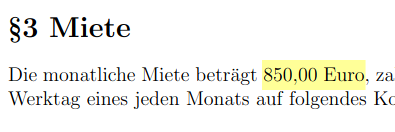
\includegraphics[width=\textwidth]{img/miete_org}
        \caption{Originales Dokument}
    \end{subfigure}
    \hfill
    \begin{subfigure}[b]{0.4\textwidth}
        \centering
        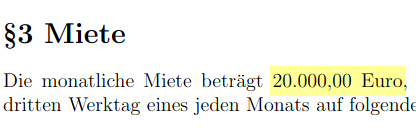
\includegraphics[width=\textwidth]{img/miete_chg}
        \caption{Verändertes Dokument}
    \end{subfigure}
    \caption{Ausschnitte aus den Mietverträgen mit Mietzins}
    \label{fig:mietvertraege}
\end{figure}
Abgesehen von dieser Änderung sind beide Dokumente identisch aufgebaut.
Ziel ist es, die beiden PDF-Dateien semantisch konsistent zu halten, während 
im Hintergrund so modifiziert wird, dass beide Dateien denselben MD5-Hashwert aufweisen.
\paragraph{Technische Umsetzung} Die MD5-Hashfunktion (Message-Digest Algorithm 5) berechnet aus einer beliebigen 
Eingabe einen 128-Bit langen Hashwert. Aufgrund des enormen Wertebereichs 
von $2^{128}$ wäre eine Kollision durch bloßes Probieren sehr aufwendig. Daher wird 
in dieser Demonstration auf eine vereinfachte Variante zurückgegriffen (Short-MD5),
bei der lediglich ein 4 Byte (32 Bit) Präfix  
der echten MD5-Hashwerte verglichen wird.
Zur Manipulation der Dateien wird deren Binärstruktur direkt verändert. 
PDF-Dateien beginnen mit einem Header, dem in der Regel Zeilenkommentare 
folgen können, die keine Auswirkungen auf den Inhalt des Dokuments haben. Diese 
Kommentare werden genutzt, um gezielt die Bytefolge zu beeinflussen:
\begin{verbatim}
%PDF-1.7
% XXXX <- Zeilenkommentar
...
\end{verbatim}
An dieser Stelle wird in beiden Dokumenten ein identischer Kommentarblock eingefügt. 
Durch automatisierte, systematische Änderungen dieses Kommentarinhalts werden 
unterschiedliche Bytefolgen erzeugt. Nach jeder Änderung wird der Hashwert berechnet 
und mit den bisherigen Einträgen verglichen. Sobald eine identische 32-Bit-Kennung 
bei beiden Dokumenten festgestellt wird, wurde eine Kollision entdeckt.
\paragraph{Code} Für die Automatisierung wurde die Programmiersprache Rust verwendet.
Zur Berechnung des verkürzten MD5-Hashs dient die Funktion \verb|short_md5|.
Dabei wird lediglich der vollständige MD5-Hash der Daten errechnet und auf die
vordersten vier Bytes reduziert.
\begin{minted}[fontsize=\small, bgcolor=bg, frame=lines, linenos]{rust}
fn short_md5<T: AsRef<[u8]>>(data: T) -> [u8; 4] {
    let digest = md5::compute(data).0; // 16 Bytes
    digest[..4].try_into().unwrap()    // 4 Bytes
} 
\end{minted}
Für die Kollisionssuche werden die zwei Dokumente $A$ und $B$ zuerst aus dem Speicher geladen und als 
Array von Bytes gespeichert.
\begin{minted}[fontsize=\small, bgcolor=bg, frame=lines]{rust}
let mut a = fs::read("./documents/mietvertrag_original.pdf")?;
let mut b = fs::read("./documents/mietvertrag_changed.pdf")?;
\end{minted}
Zur Speicherung der bereits entdeckten Hashwerte wird eine HashMap verwendet, mit
den 4 Byte Hashes als Key und den dazugehörigen Änderungen des Dokuments als Values.
\begin{minted}[fontsize=\small, bgcolor=bg, frame=lines]{rust}
let mut a_map: HashMap<[u8; 4], u32> = HashMap::new();
let mut b_map: HashMap<[u8; 4], u32> = HashMap::new();
\end{minted}
Innerhalb der PDF-Dokumente wurde wie erwähnt ein Zeilenkommentar mit 'XXXX' als 
Platzhalter eingefügt. Die vier Zeichen entsprechen genau vier Bytes und somit einem
\verb|unsigned integer|. Das erste 'X' ist in diesem Fall das elfte Byte der beiden Dokumente.
Um alle möglichen Varianten systematisch durchzugehen, wird von $0\dots 2^{32} - 1$ iteriert
und die binäre Darstellung der Dezimalzahl statt dem Platzhalter in beide Dokumente eingefügt.
\begin{minted}[fontsize=\small, bgcolor=bg, frame=lines]{rust}
for i in 0..u32::MAX {
    a[11..11 + 4].copy_from_slice(&i.to_be_bytes());
    b[11..11 + 4].copy_from_slice(&i.to_be_bytes());
    // ...
}
\end{minted}
Nach der Änderung des Platzhalters wird der Short-MD5 Hash der beiden Dokumente
berechnet.
\begin{minted}[fontsize=\small, bgcolor=bg, frame=lines]{rust}
    let a_digest = short_md5(&a);
    let b_digest = short_md5(&b);
\end{minted}
Jetzt wird in den HashMaps nach den neuen Hashwerten gesucht. Falls einer der
Werte bereits in der HashMap des anderen Dokuments ist, so wurde eine Kollision entdeckt.
Dann kann das Dokument mit dem Wert, der den gleichen Hash erzeugt hat, aus der
HashMap verändert werden. Sei beispielweise der neue Hashwert von Dokument $B$ bereits
in der HashMap von Dokument $A$ (selbiges in die andere Richtung):
\begin{minted}[fontsize=\small, bgcolor=bg, frame=lines]{rust}
    if let Some(modification) = a_map.get(&b_digest) {
        println!("Found Collision! {:?}", modification);
        a[11..11 + 4].copy_from_slice(&modification.to_be_bytes());
        break;
    }
\end{minted}
\paragraph{Ergebnis}
Durch den Algorithmus konnten die beiden Dokumente so angepasst werden, dass der
gleiche Short-MD5 Hashwert nach ungefähr 87000 Iterationen ($\approx 20,5$ ms) entsteht.
\begin{verbatim}
                (Short-MD5)     (MD5-Rest)
Original:       7bd80b59        fa50ae16acf3770f74bd6a69
Changed:        7bd80b59        db7b3913e7de464f993a2db9
\end{verbatim}
\begin{figure}[h]
    \centering
    \begin{subfigure}[b]{0.4\textwidth}
        \centering
        
\includegraphics[width=\textwidth]{img/org_adjusted}
        \caption{Originales Dokument mit angepassten Platzhalter}
    \end{subfigure}
    \hfill
    \begin{subfigure}[b]{0.4\textwidth}
        \centering
        
\includegraphics[width=\textwidth]{img/chg_adjusted}
        \caption{Verändertes Dokument mit angepassten Platzhalter}
    \end{subfigure}
    \caption{Ausschnitte aus der Textrepräsentation der beiden veränderten Dokumente}
    \label{fig:adjusted_mietvertraege}
\end{figure}
\paragraph{Fazit}
Aufgrund des Geburtstagsparadoxon lassen sich bei der vereinfachten MD5 Variante
schnell zwei gleiche Hashwerte für die Dokumente finden. Für die volle Länge
von MD5 Hashwerten würde die Suche allerdings beträchtlich länger dauern. 

\end{document}
